\documentclass[12pt]{extarticle}

\usepackage{mathptmx,helvet,courier,bm}
\usepackage{amsmath,amssymb,stmaryrd}
\usepackage[sort&compress,numbers]{natbib}
\usepackage{url}
\usepackage{graphicx}
\usepackage{longtable}
\usepackage{fullpage}
\usepackage{setspace}



\setcounter{bottomnumber}{2}

% Personal commands
%
\newcommand{\equationname}{equation}

% Demarcate figures
\newcommand{\topfigrule}{\relax\noindent\rule[-6pt]{\columnwidth}{.4pt}}
\newcommand{\botfigrule}{\relax\noindent\rule[16pt]{\columnwidth}{.4pt}}

%
% A more standardized way of making paper titles
%
\author{Jacob Calder\footnote{jcalder@utexas.edu}, Iwo Dubaniowski \footnote{mduban@gmail.com}, C. Vic Hu \footnote{vic@cvhu.org}, Subhashini Venugopalan\footnote{vsubhashini@utexas.edu}\\[4pt]
\-\\
EE380L Data Mining\\
University of Texas at Austin\\
\url{https://github.com/cvhu/ee380l-ghosh-project}
}
\title{Mining for Spillovers in Patents}

\begin{document}
\sloppy

\maketitle
%\doublespace
\onehalfspace

\begin{center}
\textbf{Abstract}
\end{center}
Knowledge spillovers

\section{Introduction}
The project proposed by Professor Rai involves analyzing a set of approximately 1000 patents that pertain to solar energy technologies obtained from the US Patent and Trademark Office\cite{us_patent}. The information provided for each patent contains the inventor(s); assignees; dates of filing, application, and issue; keywords based on standard patent classifications; geographical location of the assignee firm or inventor; etc. The patents have been pre-classified based on the portion of the supply chain the patents apply to. Additionally, the data has undergone simple topic modeling/LDA analysis based using the MAchine Learning for LanguagE Toolkit (MALLET) Java-package\cite{mallet}.

The overall goal of the project is to develop a method of clustering the patents that will allow for the discovery of temporal and spatial connections between groups of patents linked to �spillovers� in innovation. In other words, it is not uncommon for an innovation to leads to other innovations. One breakthrough that will quickly be implemented into other problems and lead to other breakthroughs. While this is intuitively easy to understand it is not easy to track or measure. Traditionally, this is tracked using citations, though this is not a reliable method because patents often cite a wide variety of other patents, many of which are not pertinent. This project will attempt to analyze the abstracts and bodies of the patents to find common phrases and attempt to use these links as a way of analyzing the spillovers from one patent to another.

\subsection{Motivation}
There is significant amount of similar work performed in the areas of copyright protection and IP portfolios management, which both also depend on models that most adequately represent patents. Consequently, there are previous works available, describing methods of textual data mining such as key phrase extraction algorithms and co-word analysis in the context of patents \cite{TLY07}. Furthermore, there are works available on evaluating these methods to best fit the problem at hand \cite{TLY03}. Moreover, the idea of textual patents similarity is a subject of an ongoing research applicable to the cognitive science and legal (patents infringements) fields resulting in different concepts of similarity measurements and similarity coefficients available \cite{MM10}.

Other than bag-of-word topic modeling, it will be interesting to analyze the writing styles and term usages between correlated patent publications. Our hypothesis assumes some underlying linguistic patterns introduced by knowledge spillover that aren't necessarily apparent in the context of citations or word frequency modeling. Although it is difficult to define and quantify such relations, we can verify our results with domain knowledges and geographical information \cite{geography}.

\subsection{Hypothesis}

	As a first step, we would like to identify and define some metrics to measure the performance of clustering with respect discovering spillovers. The most challenging aspect of the project is to come up with a language model to represent the patents. We will begin by attempting to apply known language models such as Bigram and Probabilistic Context Free Grammar (PCFG)  for topic modeling. We will then cluster the patents and attempt to find links between the clusters and patents within individual clusters and verify the performance based on the defined metrics.

The expected outcome of the project is to identify a language model (or a combination of models) and clustering techniques that can best capture knowledge transfer and spillover. The end result is intended to be a general method that can find connections between patents regardless of type of technology as well as an analysis of the provided solar power patents.


\section{Data}
\subsection{Source}

\subsection{Preprocessing}

\subsection{Chanllenges}
\newpage
\section{Background}

Given a collection of text-based patent documents, one intuitive idea to find out knowledge spillovers is to look at some underlying thematic structures hidden in the text. Based on the word usages and terminology distributions, we need to know what are the intrinsic topics implied in the relevant context, and one common way to do exactly that is called Probabilistic Topic Models formalized by  Blei et al. \cite{blei2011}

\subsection{Probabilistic Topic Models}
Originally designed to facilitate text data visualization and browsing, 

The main objective of topic modeling is to automatically discover the unobserved hidden structure--the topics, per-document topic distributions, and the per-document per-word topic assignments, with a collection of text documents as the only observable variables. 

\begin{figure}[h]
	\center	
	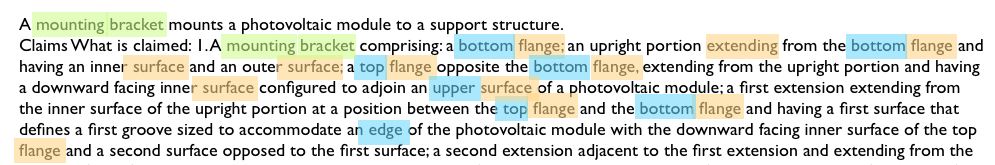
\includegraphics[width=\textwidth]{fig/pat007.png}
	\caption{A sample patent document (partial)}
	\label{sample_patent}
\end{figure}

For example, given a sample patent text, we assume that there is a set of topics associated with this patent. In Fig.~\ref{sample_patent}, we have annotated a selection of words, with each topic distinguished by colors. For the orange topic, we get words such as flange, surface and extending, which could be interpreted as having something to do with attachment of hardware components such as pipes and cylinders. Similarly, the blue and green topics could be interpreted as installation and mounting respectively. By looking at the text, any human being with average comprehensive ability can easily tell what a document like Fig.~\ref{sample_patent} is about, and highlight the associated keywords that defines such topics. 

Nonetheless, when we scale up the size and complexity of such patent documents, using human labor to do such tasks suddenly becomes erroneous and expensive. The goal of probabilistic topic modeling is to automate this process and to provide hidden insights and meaningful intelligence of big data. If we can successfully construct a reasonable thematic structure from our patent data, we can presumably infer influences or spillovers of patent authors within the same topics




\subsection{Latent Dirichlet Allocation}
Latent Dirichlet allocation, or LDA, is the simplest topic model \cite{lda2003} that assigns each word in the documents a distribution over a fixed number of topics. Instead of having a hard boundary between topic collections, LDA provides a distribution of topics per document, giving the likelihood of a mixed proportion of topic assignments. Namely, all patent documents share the same set of topic collection but with different proportions to each topic. For instance in Fig.~\ref{topic_proportion}, although there are $K=100$ topics overall, only a few topics were actually activated.

\begin{figure}[h]
	\center
	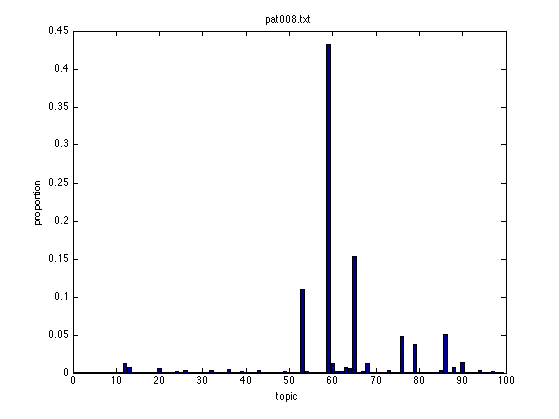
\includegraphics[width=0.55\textwidth]{fig/pat8_topics.png}
	\caption{A sample topic proportion of a patent}
	\label{topic_proportion}
\end{figure}


To build the generative probabilistic model, we compute the joint distribution and use it to estimate the posterior probability. Before jumping into the actual calculation, let's formalize our notations:

\begin{description}
	\item [$\beta_k,\; k = 1 \cdots K$]: the K topics, represented by a distribution over words
	\item [$\theta_d,\; d = 1 \cdots D$]: topic proportions for document d, where $\theta_{d,k}$ is the topic proportion of topic k for document d
	\item [$z_d,\; d = 1 \cdots D$]: topic assignments for document d, where $z_{d,n}$ is the topic assignment for the n-th word in document d
	\item [$w_d,\; d = 1 \cdots D$]: observed words for document d, where $w_{d,n}$ is the n-th word in document d
\end{description}

With the above notation, the LDA generative process can be formalized as the following joint probability of both hidden and observed random variables:

\begin{equation*}
	p(\beta_{1:K}, \theta_{1:D}, z_{1:D}, w_{1:D})\\
	= \prod_{i=1}^K p(\beta_i)\prod_{d=1}^D p(\theta_d) \left( \prod_{n=1}^N p(z_{d,n} | \theta_d) p(w_{d,n} | \beta_{1:K}, z_{d,n})\right)
\end{equation*}

which can alternatively be expressed as a graphical model:
\begin{figure}[h]
	\center
	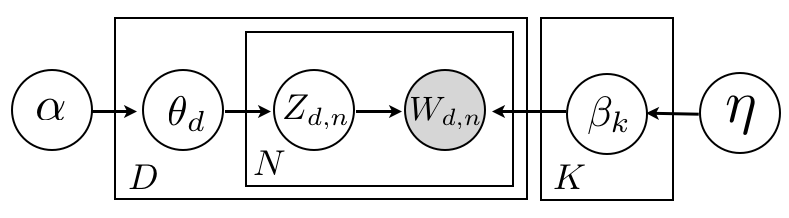
\includegraphics[width=0.75\textwidth]{fig/gm.png}
	\caption{LDA graphical model. Nodes represent variables, while edges indicate the dependency relations. The shaded node is the only observed variable (document words), and all others are the hidden variables. The $D$ plate denotes the replicated variables product over $D$ documents, while the $N$ plate denotes replication over $N$ words in each document.}
	\label{graphical_model}
\end{figure}

Note that there are several conditional dependencies implied in the graphical models, which reflects the main principles of how LDA ``think'' the documents are generated:

\begin{enumerate}
\item Randomly pick a distribution $\theta_d$ over topics.
\item For each word in the document
	\begin{enumerate}
	\item Randomly choose a topic from the previously-chosen distribution $\theta_{d,n}$.
	\item Randomly choose a word from the corresponding distribution $Z_{d,n}$.
	\end{enumerate}
\end{enumerate}

Assuming this generative process is how our documents are created, now LDA uses the graphical model in Fig.~\ref{graphical_model} to infer the posterior probability of the hidden structures given our observable:

\begin{equation*}
p(\beta_{1:K}, \theta_{1:D}, z_{1:D} | w_{1:D}) = \frac{p(\beta_{1:K}, \theta_{1:D}, z_{1:D}, w_{1:D})}{p(w_{1:D})}
\end{equation*}

The computation of possible topic stuctures is often intractable and the posterior distribution can only be approximated in most cases. To form an approximation algorithm, topic modeling can generally be categorized as sampling-based algorithms and variational algorithms. The most popular sampling method for topic modeling is Gibbs sampling, which introduces a sequence of random variables to construct a Markov chain and collects samples from the limiting distribution to estimate the posterior. Instead of using samples to approximate the posterior, variational methods find the closest parameterized distribution candidate by solving optimization problems \cite{lda2003} \cite{bach2010}.

\begin{figure}[h]
	\center
	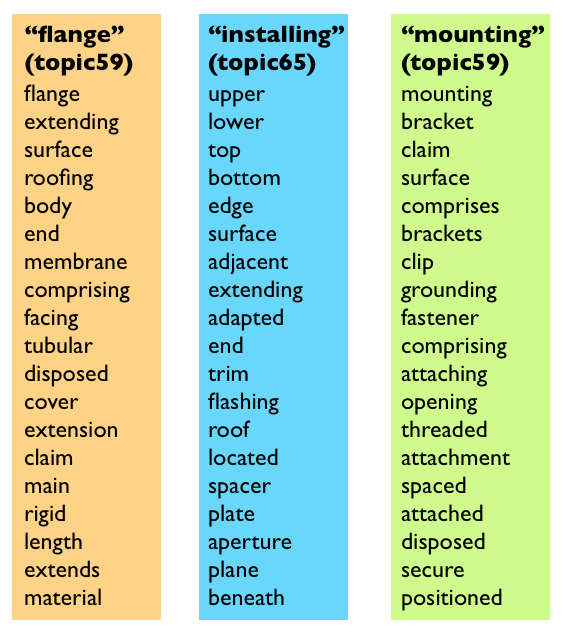
\includegraphics[width=0.5\textwidth]{fig/topics.png}
	\caption{The top 3 topics of a sample patent}
	\label{top3topics}
\end{figure}





\subsection{Limitations \& Potential Improvements}
Although LDA provides a powerful perspective to browsing and interpreting the implicit topic structures in our patent corpus, there are a few limitations it imposes against further discoveries. An extensive amount of research has been focused on relaxing some of the assumptions made by LDA to make it more flexible and suitable for various adaptations in different context. 

\begin{description}
	\item[Bag of Words] LDA is essentially a bag-of-words probabilistic model. Namely, it constructs a word frequency vector for each document but disregards the word ordering or the surrounding context. Although this assumption looses the syntactic information and sometimes seems unrealistic when processing natural language, it is usually good enough when capturing the document semantics and simplifying hidden structural inferences. Nonetheless, for more sophisticated tasks such as language generation or writing style modeling, the bag-of-words assumption is apparently insufficient and needs to be relaxed. In such cases, there are variants of topic models that generate topic words conditional on the previous word \cite{wallach2006}, or switches between LDA and hidden Markov models (HMM) \cite{griffiths2005}.
	\item[Document Ordering] The LDA graphical model in Fig.~\ref{graphical_model} is invariant to the ordering of our patent documents, which could be inappropriate if the hidden thematic structure is actually dependent on sequential information such as years published, which is typical in document collections spanning years, decades or centuries. To discover how the topics change over time, the dynamic topic model \cite{blei2006} treats topics as a sequence of distributions over words and tracks how they change over time.
	\item[Fixed Number of Topics] In either LDA or more sophisticated dynamic topic models \cite{blei2006}, the number of topics $\beta_{1:K}$ is determined manually and assumed to be fixed. One elegant approach provided by the Bayesian nonparametric topic model \cite{teh2006} is to find a hierarchical tree of topics, in which new documents can now imply previously undiscovered topics.
	\item[Meta-data] To include additional attribute information associated with the documents such as authorships, titles, geolocation, citations and many others, an active branch of research has been performed to incorporate meta-data in topic models. The author-topic model \cite{rosen-zvi2004} associates author similarity based on their topic proportions, the relational topic model \cite{blei2010} assumes document links are dependent on their topic proportion distances, and more general purpose methods such as Dirichlet-multinomial regression models \cite{mimno2008} and supervised topic models \cite{blei2007}.
	\item[Others] Many other extensions of LDA are available, including the correlated topic model \cite{blei2007a}, pachinko allocation machine,  \cite{li2006}, spherical topic model \cite{reisinger2010}, sparse topic models \cite{wang2009} and bursty topic models \cite{doyle2009}.
\end{description}

\subsection{MALLET}
The Java-based package we used for topic model training is called MAchine Learning for LanguagE Toolkit (MALLET), developed by the team led by McCallum at the University of Massachusetts Amherst \cite{mallet}. It covers various algorithms for statistical natural language processing, document classification, clustering, topic modeling, information extraction and many other text-based machine learning applications, including Hidden Markov Models (HMM), Conditional Random Fields (CRF), decision trees and others. More importantly, the MALLET topic modeling toolkit provides sample-based implementations of LDA, pachinko allocation and Hierarchical LDA.

\newpage
\section{Methodology}
The methodology we decided to use involved few carefully planned stages that put together will eventually produce reasonable results in terms of patent classification and knowledge spillover patterns in the field of solar energy. As mentioned previously we have focused on applying primarily methods of clustering to our solutions. The main tool that we used during the course of this project is MALLET (Machine Learning for Language Toolkit) discussed in previous sections. The main features supplied by MALLET that we used are Topic Modelling and Clustering. MALLET toolkit is an open source project developed by the University of Massachusetts � Amherst.

As we began working on the project, it became clear that the best way of tackling the problem is clustering, the nature of knowledge spillover is such that at the beginning there is no much data given on how the knowledge is being transferred from one field to another. This ruled out classification or regression methods at least in the initial stage. Furthermore, we decided to choose MALLET as the package that we will be working with. It provides very good tools for language and textual analysis and is easy in use and access, being written in Java and open source. Having many features, MALLET will allow us to try different approaches to tackling the problem and to limit the need to use other outside tools.

The data we used was supplied to us by a research group for the knowledge spillover in solar energy field working under Dr Rai. The database we received was handpicked by this group and one of our major concerns is how to approach handling these data. We ended up accessing United States Patent and Trademark Office (USPTO) website in order to get fuller and better representation of the data that we had obtained.

The above paragraphs show the biggest concerns and the main decisions we had to make in regards to the methodology that we used throughout this project. After deciding these key factors we could concentrate on actual use of these resources in order to come up with a method to find out patterns in the knowledge spillover.

First, issue that we encountered and that we had to spend considerable amount of time on is cleaning up the data and deciding which parts of patent texts are the most suitable to use for the task at our hands. We concluded that the best sections of patent documents to base spillover patent prediction are abstracts and claims. Abstracts show the shortest and most concise understanding of what the patent is about and therefore seem to be perfect for our needs. However, abstracts are usually not long, in terms of text size, enough to present on their own a considerable value in data mining applications and therefore they need to be supplemented. The best choice for the supplementary field turned out to be �claims� as they are the heart of the patent that in contrary to description or citations fields does not talk about previous or other patents and topics. Patent�s citations often contain redundant entries that are presented only to cover the patent to the fullest from the legal perspective. Similarly, description often involves the whole historical and technical background of the patent that is not something that we are interested in. Therefore, we decided to use the two patent document fields in our project, namely, abstract and claims.

To obtain these fields, a web crawling script was written in Java that crawled USPTO�s website in order to get the required data. The script used patent number in case of patents and application number in case of application to access the right entry. At this point abstract and claims fields were extracted from the entry to form the final entry that will be used from now on. The main difficulties with this step were different formats of application and patent numbers that did not work well with our script. Similarly, some patents had this number not provided, instead they had �publication number�, in these cases we had to get the right number first before crawling. Also, the navigation of USPTO website search engines is fairly complicated so getting accustomed to that took us awhile too.

After obtaining the data, the next step was to run topic modelling on the texts that we had obtained earlier. The details of what is topic modelling is have been provided in earlier paragraphs, so I will just briefly state how we applied topic modelling to our datasets. The data for each patent, i.e. abstract and claims, has been put into a separate file. Later all these files were supplied to MALLET together with standard �stop words� list in English language list to perform the topic modelling on the data. When running topic modelling we tried to come up with different values of �n� � the number of topics created. After few runs and analysis of the outputs created, we decided that �n� equal to 10 is the most reasonable option. Furthermore, since topic modelling in MALLET is not deterministic, we ran the modelling with n=10 few times to make sure that this is the right choice and to arrive with the best range of topics.

Following the topic modelling we assigned each topic a very general class that it represented by looking at the topic models themselves. The classes we used for this purpose were �SolarInventer�, �Solar Mounting/Rack�, �Solar Monitoring� and �Site Assesment�. An example of a topic model can be seen on Fig. 1. It is the least of word in order of frequency as theyappear in each topic. This topic model was ran for n=15. To assign a class to a topic we looked at the list of words and arbitrarily decided which class given topic fits the most.

Next step was evaluating our results in attempt to see whether the topic models we arrived with are reasonable and reflect the actual patents distribution well. To approach this task we had to come up with a method that would compare our classes to some other method of classification. Since patent applications that arrive to USPTO are given classes by patent officers as they are filed we decide to use one of these as our method of evaluation. The patent classification scheme we decided to use is CPC � Cooperative Patent Classification. Each patent is assigned one or more CPC classes as its application is filed to USPTO and we used these classes to see whether our topic models constitute a valid solution.

After ensuring that the topic models make sense we went on and grouped the data by geographies. Outside of the US it was done by continents. This is due to the fact that overwhelming number of patents unsurprisingly came from inside the US, the distribution of patents by countries can be seen on Fig. 2. Inside the US the clustering was done based on regions and states. We divided California into two regions, Bay Area and Southern California due to a great number of patents originating in that state. Following that we classified patents using our topic models obtained earlier into these topics. This gave us an opportunity to see which topics are popular in which areas and to form conclusions on whether certain topics are more popular in given geographies implying knowledge sharing and spillover.

Similarly, we divided patents by years and subsequently classified them into topics to see in which they were filed to see whether there are patterns of topics being more popular during certain time periods. This task was more difficult due to the fact that solar technology innovation field is very new and there is not many patents from the beginnings of the time period (2006-2012) we are working on. On Fig. 3 we can see all patents grouped by year and technology area, before running topic modelling on them.

Following the two procedures above we checked whether topics divisions inside the groups are relevant by seeing how much they overlap with CPC classes of the patents. This step was performed to ensure that our topic models, even when patents are divided into groups by geographies or years, still make sense and represent the actual topics that patents relate to.

Finally, the last step was to visualize the data to notice any patterns in knowledge spillover in the field of solar energy. It is much easier to see these patterns visually than in numerical and textual form. This allowed us to find any trends in the distribution of the topics and possibly to find out whether we can use data mining techniques to see whether and to what extent there is knowledge spillover in solar energy technology field. Next part of this paper will attempt analyse the results that we have arrived with.
%\section{}

\section{Results}

\section{Conclusion}

\section{Future Works}



\begin{thebibliography}{1}

\bibitem{us_patent}
The United States Patent and Trademark Office, http://www.uspto.gov/patents/process/search/. 2012
\bibitem{mallet}
McCallum, Andrew Kachites.  "MALLET: A Machine Learning for Language Toolkit."
    http://mallet.cs.umass.edu. 2002.
\bibitem{TLY07}
Yuen-Hsien Tseng, Chi-Jen Lin, Yu-I Lin. Text mining techniques for patent analysis. Information Processing and Management, Volume 43, Issue 5, September 2007. http://www.sciencedirect.com/science/article/pii/S0306457306002020
\bibitem{TLY03}
Tao Liu, Shengping Liu, Zheng Chen, and Wei Y. Ma. �An evaluation on feature selection for text clustering. 
	Proc. 20th International Conference on Machine Learning (ICML03), August 2003.
\bibitem{MM10}
Martin Moehrle. Measures for textual patent similarities: a guided way to select appropriate approaches. Scientometrics, May 2010. 
	http://link.springer.com/article/10.1007\%2Fs11192-010-0243-3?LI=true\#
\bibitem{geography}
Peter Thompson. Patent Citations and the Geography of Knowledge Spillovers: Evidence from Inventor- and Examiner-added Citations The Review of Economics and Statistics. 2006

\bibitem{blei2011}
Blei, D. Introduction to Probabilistic Topic Models. Princeton University. 2011.

\bibitem{lda2003}
Blei, D., Ng, A. and Jordan, M. Latent Dirichlet allocation. Journal of Machine Learning Research, 3:993-1022, January 2003.

\bibitem{bach2010}
Hoffman, M., Blei, D. and Bach, F. On-line learning for latent Dirichlet allocation. In Neural Information Processing Systems, 2010.

\bibitem{wallach2006}
Wallach, H. Topic modeling: Beyond bag of words. In Proceedings of the 23rd International Conference on Machine Learning, 2006.

\bibitem{griffiths2005}
Griffiths, T., Steyvers, M., Blei, D. and Tenenbaum, J. Integrating topics and syntax. In L. K. Saul, Y. Weiss, and L. Bottou, editors, Advances in Neural Information Processing Systems 17, pages 537-544, Cambridge, MA, 2005. MIT Press.

\bibitem{blei2006}
Blei, D. and Lafferty, J. Dynamic topic models. In International Conference on Machine Learning, pages 113-120, New York, NY, USA, 2006. ACM

\bibitem{teh2006}
Teh, Y., Jordan, M., Beal, M. and Blei, D. Hierarchical Dirichlet process. Journal of the American Statistical Association, 101(476):1566-1581, 2006.

\bibitem{rosen-zvi2004}
Rosen-Zvi, M., Griffiths, T., Steyvers, M. and Smith, P. The author-topic model for authors and documents. In Proceedings of the 20th Conference on Uncertainty in Artificial Intelligence, pages 487-494. AUAI Press, 2004.

\bibitem{blei2010}
Chang, J. and Blei, D. Hierarchical relational models for document networks. Annals of APplied Statistics, 4(1), 2010.

\bibitem{mimno2008}
Mimno, D. and McCallum, A. Topic models conditioned on arbitrary features with Dirichlet-multinomial regression. In Uncertainty in Artificial Intelligence, 2008.

\bibitem{blei2007}
Blei, D. and McAuliffe, J. Supervised topic models. In Neural Information Processing Systems, 2007.

\bibitem{blei2007a}
Blei, D. and Lafferty, J. A correlated topic model of Science. Annals of Applied Statistics, 1(1):17-35, 2007.

\bibitem{li2006}
Li, W. and McCallum, A. Pachinko allocation: DAG-structured mixture models of topic correlations. In International Conference on Machine Learning, pages 577-584, 2006.

\bibitem{reisinger2010}
Reisinger, J., Waters, A. ,Silverthorn, B. and Mooney, R. Spherical topic models. In International Conference on Machine Learning, 2010.

\bibitem{wang2009}
Wang, C. and Blei, D. Decoupling sparsity and smoothness in the discrete hierarchical dirichlet process. In Y. Bengio, D. Schuurmans, J. Lafferty, C. K. I. Williams, and A. Culotta, editors, Advances in Neural Information Processing Systems 22, pages 1982-1989. 2009.

\bibitem{doyle2009}
Doyle, G. and Elkan, C. Accounting for burstiness in topic models. In International Conference on Machine Learning, pages 281-288. ACM, 2009.

\end{thebibliography}
%

\end{document}  
